\Extrachap{Solutions}

\section*{Problems of Chapter~\ref{intro}}

\begin{sol}{prob1}
  \begin{enumerate}
    
\item A proton with an energy of 450~MeV has a momentum of:
  $$ p = \sqrt{(T+m_p)^2-m_p^2)} = 1023~{\rm MeV}$$

 Given that $p \, (GeV) = 0.3 B \, (T) \rho \, (m)$, in order to achieve a radius of curvature of 1.9~m, the magnetic field needed is: 
  $$ B = \frac{p}{0.3 \rho} = 1.8~{\rm T} $$

\item The energy and momentum of the pions are:

  $$E_{\pi^-} = 100 + 139 = 239~\rm{MeV}$$
  $$p_{\pi^-} = \sqrt{E_{\pi^-}^2 - m_{\pi^-}^2} = 194.4~\rm{MeV}$$

  Therefore the centre of mass energy will be:

  $$ \sqrt{s} = \sqrt{(E_{\pi^-}+m_p)^2-p_{\pi}^2} = 1161~{\rm MeV}$$

\item Starting from:

  $$ \sqrt{s} = 1232~{\rm MeV} = \sqrt{(E_{\pi^-}+m_p)^2-p_{\pi^-}^2} $$

  and then

  $$ T_{\pi^-} = \frac{m_{\Delta}^2 - m_p^2 -m_{\pi^-}^2}{2m_p} - m_{\pi^-} = 190~{\rm MeV} $$

\item In the centre of mass of the resonance, the energy of the pion can be evaluated as:

  $$ E_{\pi^0}^* + E_n^* = m_{\Delta}$$ 
  $$ p_{\pi^0}^* + p_n^* = 0$$ 

  then:
  
$$ E_{\pi^0}^* = \frac{m_{\Delta}^2+m_{\pi^0}^2-m_n^2}{2m_{\Delta}} = 265~{\rm MeV} $$ 

  and therefore

$$  p_{\pi^0}^* = \sqrt{E_{\pi^0}^*-m_{pi^0}} = 228~{\rm MeV/c} $$ 

Taking as axis of reference the initial direction of the beam of pions, and the polar angle defined as the angle between the direction of the neutral pion and this axis:

$$(E_{\pi}^*, p_{\pi}^* \cos \theta^*, p_{\pi}^* \sin \theta^*, 0)$$

  Being that the initial momentum of the resonance $\Delta$ is the momentum of the $\pi^-$, the velocity of the centre of mass system is:
  
  $$\beta_{cdm} \gamma_{cdm} = |\vec{p_{\pi^-}}|/m_{\Delta} = 0.242$$

  and therefore:

  $$ \gamma_{cdm} = \sqrt{|\vec{p_{\pi^-}}|^2/m_{\Delta}^2+1} = 1.029$$
  
  
  The quadri-momentum in the laboratory reference frame can be obtained from the inverse Lorentz transformation (of the boost of the centre of mass), that is:

  $$  E_{\pi^0} = \gamma_{cdm} E_{\pi^0}^* + \beta_{cdm} \gamma_{cdm} p_{\pi^0}^* $$

  Therefore the maximum energy is obtained for $\cos \theta^* = 1$ and the minimum energy for $\cos \theta^* = -1$, being:

  $$ T_{\pi^0}^{max} = 192.6 \, {\rm MeV} $$
  $$ T_{\pi^0}^{min} = 82.3 \, {\rm MeV} $$
  
\end{enumerate}

The solution\index{problems}\index{solutions} is revealed here.
\end{sol}


\begin{sol}{prob2}
\textbf{Problem Heading}\\
(a) The solution of first part is revealed here.\\
(b) The solution of second part is revealed here.
\end{sol}



\vspace{0.5cm}
1. {\it Relativistic Doppler effect and the Ives and Stilwell experiment}
\vspace{0.5cm}

A light source emits photons with a frequency of $\nu_s$ in the $x$ direction.
The source is moving towards the observer as it is shown in Figure~\ref{Doppler1}.

\begin{figure}[h]
\centering
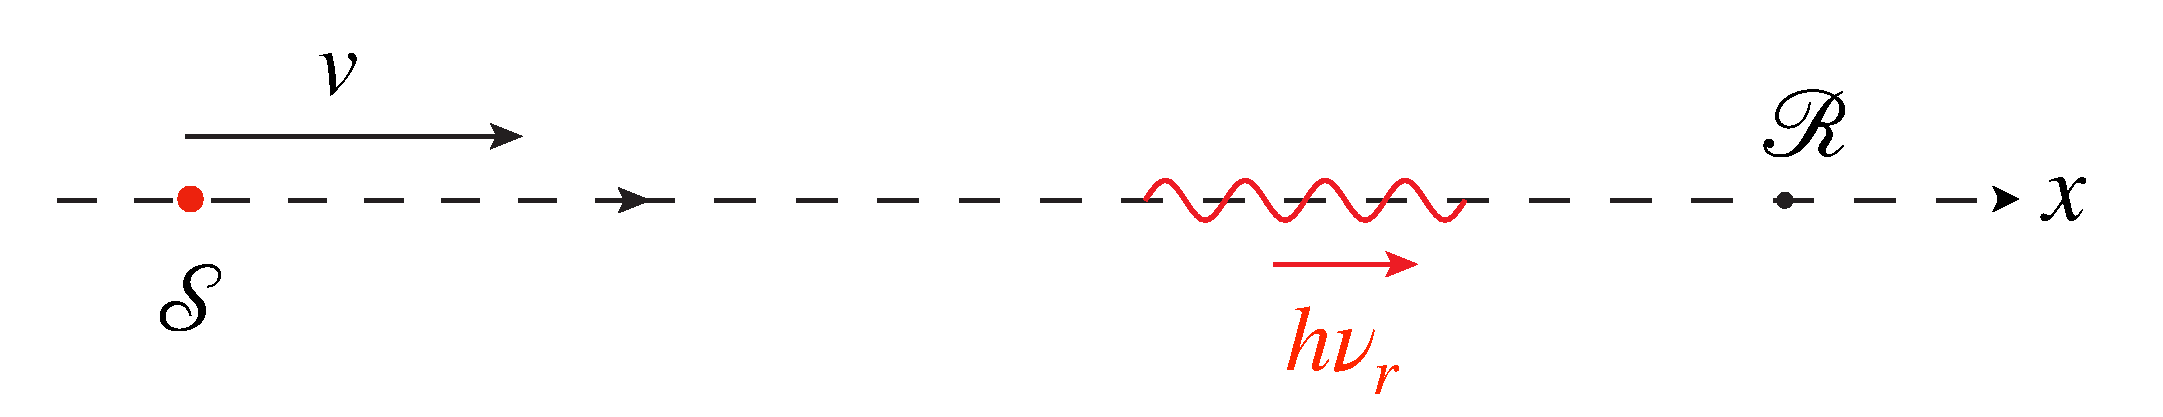
\includegraphics[width=0.7\textwidth]{Figures/Scritto-Ia.pdf}
\vskip -0.2cm
\caption{\label{Doppler1} Illustration of an emitted photon with momentum $h\nu_r$ (in the reference frame of the observer or receiver
  $\mathcal{R}$), in case of a monochromatic source $\mathcal{S}$ which is moving with an uniform straight motion in the direction of the observer.}
\end{figure}

\begin{enumerate}

\item Starting from the transformation of the quadri-momentum, evaluate the observed frequency $\nu_r$ by an observer while the light source is moving with velocity $v$ in the direction $x$.

\item Accelerating protons with a machine which is reaching a voltage of 40 kV, which is their velocity and their kinetic energy?

\begin{figure}[ht]
\centering
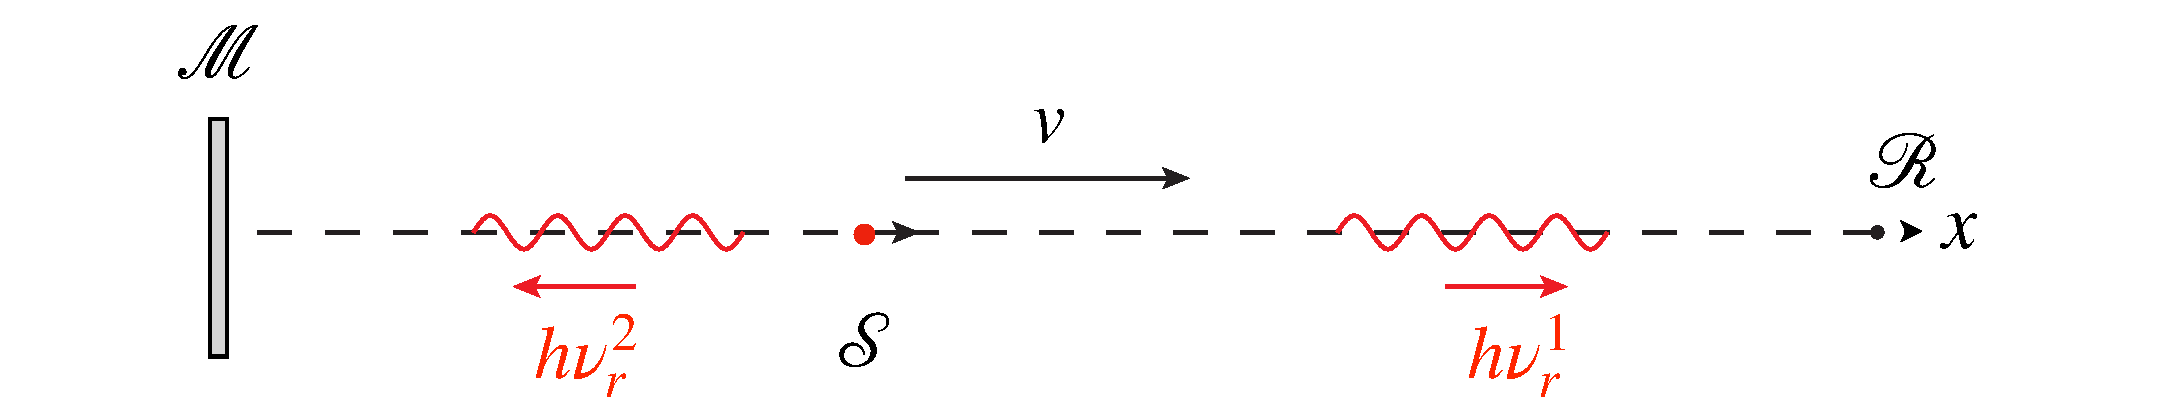
\includegraphics[width=0.7\textwidth]{Figures/Scritto-Id.pdf}
\vskip -0.2cm
\caption{\label{Doppler3} Illustration of the experiment of Ives and Stilwell, where the photon is emitted by the source ($\mathcal{S}$) has a momentum $h\nu_r^1$ when moving towards the observer (in the reference frame of the observer $\mathcal{R}$) and $h\nu_r^2$ when it is moving in the opposite direction. The latter is reflected by a mirror in $\mathcal{M}$ and then measured by an observer in in $\mathcal{R}$.}
\end{figure}

\item In air protons capture electrons to form excited hydrogen atoms and emits photons with a wave length $\lambda = 656.3$~nm (first line of Balmer $\alpha$, noted $H_{\alpha}$). Ives and Stilwell had the idea to perform this experiment by introducing a mirror which could reflect the light emitted in the opposite direction with respect to the position of the observer, and allowed the measurement of the wave lengths between the photons emitted in the $x$ direction and in the opposite one, as it is shown in Figure~\ref{Doppler3}. Which is the frequency difference between the $H_{\alpha}$ radiation emitted in the flight direction of the Hydrogen atom and the one emitted in the opposite direction?

  \vspace{0.5cm}
  
  {\it This experiment has been fundamental to demonstrate the existence of the Doppler effect for light in vacuum.}\\

\begin{figure}[h]
\centering
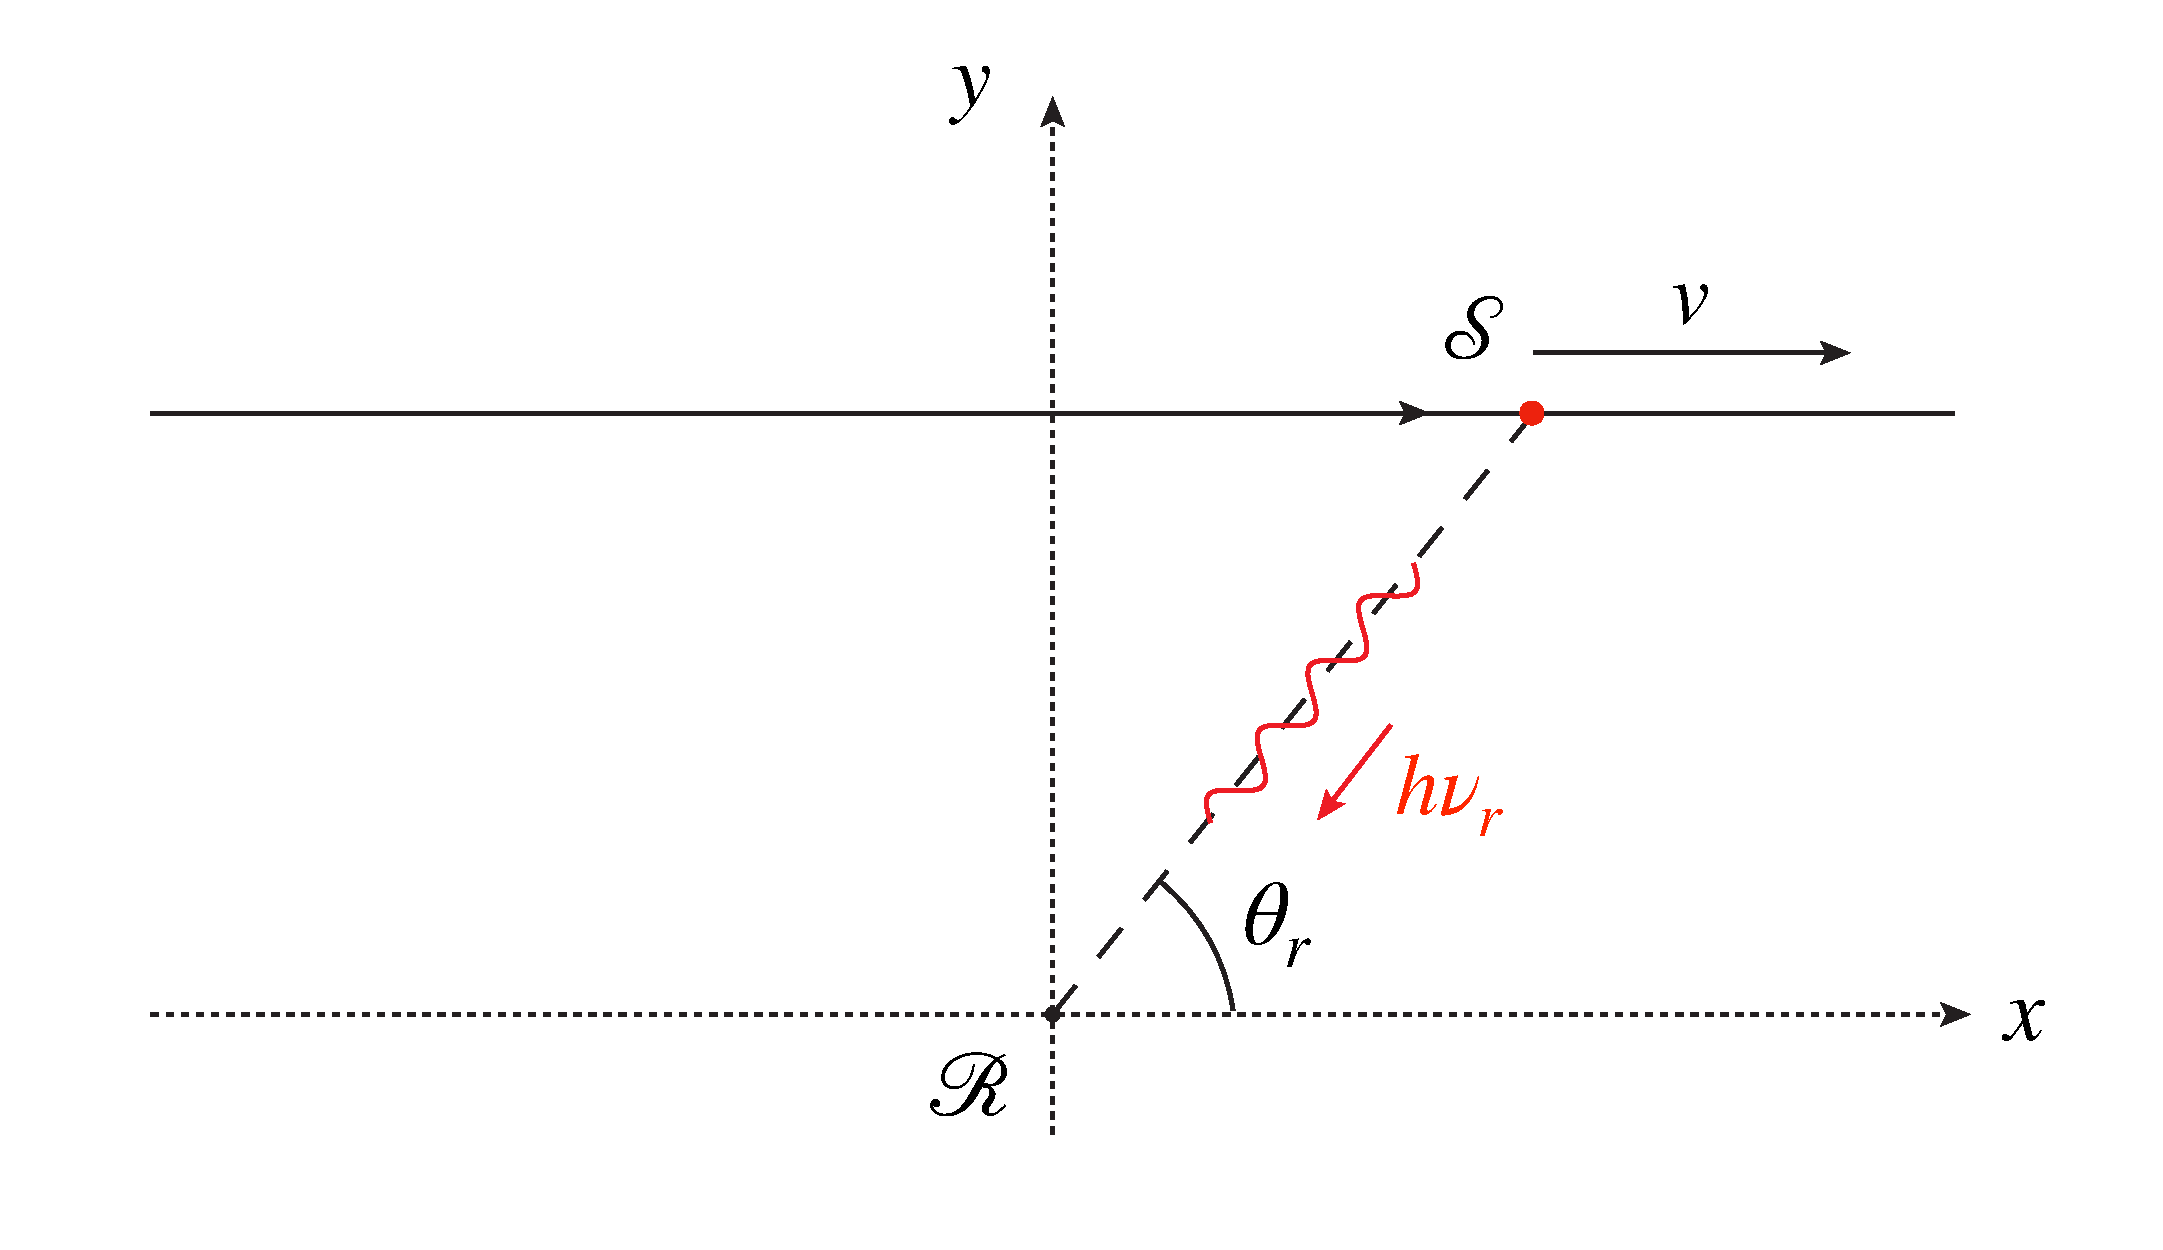
\includegraphics[width=0.7\textwidth]{Figures/Scritto-Ib.pdf}
\vskip -0.2cm
\caption{\label{Doppler2} Illustration of a photon emitted with momentum $h\nu_r$ (in the reference frame of the observer or receiver  $\mathcal{R}$), in case of a monochromatic light source $\mathcal{S}$
which is moving with a uniform straight motion in a non colliding course with the observer.}
\end{figure}

\item The evaluated effect is the longitudinal relativistic Doppler effect. Consider a light source which is moving with a uniform straight motion in a non colliding course with respect to an observed, as it is shown in Figure~\ref{Doppler2}. Evaluate the analytical form of the frequency $\nu_r$ observed as a function of the emitted frequency $\nu_s$, of the angle $\theta_r$ and of the velocity of the source ($\beta$).

\item Which is, in the reference frame of the observer, the frequency of the observed photon received in the {\it spatial} point in which the observer {\bf sees} the source at the point of minimum distance (an observation exactly perpendicular to the relative motion of the source)?
  
\item Which is the frequency of the photon observed when the source and the observer {\bf are} at the point of minimum distance? Which will be the observation angle $\theta_r$ in this case?

\item In the reference frame of the observer, which is the observation angle (which indicates the position of the source at the moment of the emission) such that the observer measures the same frequency of the light at the time of the emission?

\end{enumerate}

\begin{solution}
  \begin{enumerate}
    
  \item The observed photon has a momentum $p_r = h\nu_r$ and an energy $h\nu_r$. For a Lorentz transformation the reference frame of the source is moving with a velocity $\beta = vc$ in the direction of the observer (which is the same of the photon momentum), therefore:

    $$h\nu_s = \gamma h\nu_r - \beta\gamma h\nu_r$$

    then

    $$\frac{\nu_s}{\nu_r} = \gamma (1-\beta) = \frac{1-\beta}{\sqrt{1-\beta^2}} = \sqrt{\frac{1-\beta}{1+\beta}}$$

   so

    $$ \nu_r = \sqrt{\frac{1+\beta}{1-\beta}} \, \nu_s $$


\item Protons emitted from a 40~kV source have $\frac{1}{2} m v^2 = eV$, which is $$v= \sqrt(2 \times 1.6 \, 10^{-19} \times 40000/1.672649 \,
  10^{-27}) = 2.8 \, 10^6$$

THerefore $\beta \sim 0.01$ and the kinetic energy:

  $$ T = E - mc^2 = (\gamma-1) mc^2 = 40~keV$$

\item Photons emitted in the direction of the observer have a measured frequency of:

  $$ \nu_r = \sqrt{\frac{1+\beta}{1-\beta}} \, \nu_s$$

  and the photons emitted in the opposite direction instead:
  
  $$ \nu_r = \sqrt{\frac{1-\beta}{1+\beta}} \, \nu_s$$
  
  therefore the difference $\Delta \lambda$ will be:

  $$\Delta \lambda = (\sqrt{\frac{1-\beta}{1+\beta}} -
  \sqrt{\frac{1+\beta}{1-\beta}}) \times \lambda \sim 12 \; {\rm nm}$$

  which is a measurable effect.

\item The quadri-momentum of the photon in the reference frame of the observer is

  $$(h\nu_r, -h\nu_r \cos \theta_r, -h\nu_r
  \sin \theta_r, 0)$$

  and the Lorentz transformation to obtain the quadri-momentum in the reference frame of the source which is moving away from the observer will be:

  $$ h\nu_s = \gamma h\nu_r - \beta \gamma (- h\nu_r \cos \theta_r) =
  h\nu_r \times \gamma (1+\beta \cos \theta_r) $$

  Therefore

  $$ \nu_r = \frac{\nu_s}{\gamma (1+\beta \cos \theta_r)} $$

  We can immediatly see that for $\cos \theta = 1$ we get the relation of (1).

\item The observed frequency will be obtained exactly for $\cos \theta_r = 0$, therefore

   $$ \nu_r = \frac{\nu_s}{\gamma} $$

  One can note that for a wave received perpendicularly to the direction of motion of the source it exists a contraction effect of the frequency (dilatation of time). For the Doppler effect of sound this effect does not exist.

\item In the reference frame of the osurce, the quadri-momentum of the emitted photon is 

  $$\begin{pmatrix}
h\nu_r \times \gamma (1+\beta \cos \theta_r) \\
h\nu_r \times \gamma (\beta  + \cos \theta_r) \\
h\nu_r \times (-\sin \theta_r)\\
0\\
\end{pmatrix}$$

Being that the minimum distance is the same in the two reference frames, when the source emits towards the observer, the quadri-momentum of the emitted photon will be:

$$\begin{pmatrix}
  h\nu_s  \\
   0 \\
   h\nu_r\\
  0\\
\end{pmatrix}$$

We can then express the ratio $\xi = \frac{\nu_s}{\nu_r}$ as:

$$ \xi = \gamma (1+\beta \cos \theta_r \; \; \; \; \; e \; \; \; \; \; \xi = \sin \theta_r$$

therefore

$$ \frac{(\xi - \gamma)}{\beta\gamma} = \cos \theta_r \; \; \; \Rightarrow \; \; \; \left ( \frac{(\xi - \gamma)}{\beta\gamma} \right )^2 = 1- \xi^2 $$

then

$$ \xi^2 (1- \beta^2 \gamma^2) - 2\gamma \xi + \gamma^2 - \beta^2 \gamma^2 \; \; \; \Rightarrow \; \; \;
(\gamma \xi)^2 - 2 (\gamma \xi) + 1 = 0 $$

therefore

$$\gamma \xi = \gamma \frac{\nu_s}{\nu_r} = 1 $$

The other solution for $\gamma \xi = -1$ is non-physical. Therefore

$$ \nu_r = \gamma \nu_s $$

The observation angle in this case will be:

$$ \cos \theta_r = (\frac{1}{\gamma^2} -1)/\beta \; \; \; \; \Rightarrow \; \; \; \; \cos \theta_r = -\beta $$

\item in this case, putting $\nu_s = \nu_r$ we obtain:

  $$ 1 = \gamma + \beta \gamma \cos \theta_r \; \; \; \; \Rightarrow \cos \theta_r = \frac{1-\gamma}{\beta\gamma} $$

  An angle within 0 and $-\beta$.

\end{enumerate}
\end{solution}


\question

The $\pi^0$ meson was discovered by studying the photo-production on protons at rest
Il mesone $\pi^0$ \`e stato scoperto studiando la fotoproduzione su $\gamma p \rightarrow \pi^0 p$, process called of Primakoff.

\begin{enumerate}

\item Evaluate the threshold energy of the photon in the laboratory to produce the reaction.

\item Which is the energy of the photon in the centre of mass reference frame of the reaction at threshold energy?
  
\item The $\pi^0$ decays mainly in two photons, which is the maximum energy of a secondary photon in the laboratory reference frame?

\item Which is the minimum energy of a photon in the laboratory reference frame in order that a secondary photon of the decay could lead to the production of an additional $\pi^0$?

\end{enumerate}
  
{\it Data} $m_{\pi^{0}} = 135$~MeV/c$^2$ e $m_{p} = 938$~MeV/c$^2$ 

{\it Additional material: J. Steinberger, W. K. H. Panofsky, and J. Steller,
“Evidence for the Production of Neutral Mesons by Photons.”
Phys. Rev., 78, 802 (1950).}


\begin{solution}
  \begin{enumerate}
    
\item Assuming that the threshold corresponds to the energy for which the energy in the centre of mass reference frame is given only by $m_{\pi^0}+m_p$ we get:

  $$ E_{\gamma}^{\rm soglia} = \frac{m_{\pi^0}^2 + 2 m_p m_{\pi^0}}{2
    m_p} = 145 \; {\rm MeV} $$

\item The velocity of the centre of mass system is $\beta = 0.1336$ and $\gamma =
  1.009$ therefore the energy of the photon in the centre of mass reference frame will be:
  
  $$ E'_{\gamma} = \gamma E_{\gamma} - \beta \gamma E_{\gamma} = 126.5 \; {\rm MeV}$$

\item The energy of one of the photons with an angle $\theta$ with respect to the initial velocity of the photon in the reference frame of the centre of mass will be.

  $$ E_{\gamma} = \frac{m_{\pi^0}}{2} (\gamma + \beta \gamma \cos \theta) $$

    therefore the maximum energy will be obtained for $\cos \theta = 1$ and therefore:

    $$ E_{\gamma}^{\rm max} = 77.2 \; {\rm MeV}$$

  \item In order to reach an energy of the secondary photon of $\tilde{E} =$145~MeV in the laboratory reference frame, the needed velocity $\beta$ can be calculated as:

    $$\tilde{E} =  \frac{m_{\pi^0}}{2} (\gamma + \beta \gamma)
    \; \; \; \; \Rightarrow \; \; \; \; (\gamma + \beta \gamma) =  \frac{2\tilde{E}}{m_{\pi^0}} \equiv a $$

    therefore

    $$ \gamma + \beta \gamma = a \; \; \; \; \Rightarrow \; \; \; \;  (1+\beta)^2 = a^2 (1-\beta^2) \; \; \; \; \Rightarrow \; \; \; \; (1+a^2) \beta^2 + 2\beta + (1-a^2) = 0$$

    The only physical solution is:

    $$ \beta = \frac{a^2-1}{a^2+1} \; \; \; \; \Rightarrow \; \; \; \; \beta = 0.64 $$

    The velocity in the centre of mass reference frame is then given by

    $$ \beta = \frac{E_{\gamma}}{E_{\gamma}+m_p} \; \; \; \; \Rightarrow \; \; \; \; E_{\gamma} = \frac{\beta}{1-\beta} m_p = 1.7 \; {\rm GeV}$$
    
    
\end{enumerate}
\end{solution}


\question

A scattering experiement of $\alpha$ particles on a gold foil is prepared. The source of $\alpha$ radiation is Americium $^{241}{\rm Am}$. Most of the $\alpha$ particles are emitted with a kinetic energy of  $E_{\alpha} = 5.496$~MeV. The source radiates uniformly in all directions with a radio activity of 1.5~mCi
(milli-Curie, where 1 Ci$ = 2.22 \, 10^{12}$~dpm -- decays per minute).\\

The source ($s$) placed in a lead container which colimates a beam of $\alpha$ particles towards the target, the distance between the circular hole and the source is $\ell_1 = 15$~cm and the collimating hole has a diameter of $d_1 =
0.5$~cm. The target is a thin gold foil ($^{79}$Au) with a thickness of 
2~$\mu$m a diameter of $d_2 = 1$~cm and placed at $\ell_2 =
5$~cm from the hole. \\ 

The detector can rotate around the target and is made of silicon. It has a circular shaped active surface area with a diameter of $d_3 =
0.5$~cm and it is placed at $\ell_3 = 15$~cm from the target.\\

The thickness of the gold foil $\mathcal{A}$ has to be determined. It can be lowered in the beam to decrease the beam energy. Its surface area is not specified, but it is large enough to cover entirely the outgoing beam. The experiment is illustrated in Fig.~\ref{Rutherford}.\\

The scattering cross section for the Rutherford scattering has been calculated as a function of the scattering angle $\theta$ and the kinetic energy $E$:

$$ \frac{d\sigma}{d\Omega} = \left ( \frac{zZ e^2}{4\pi \varepsilon_0}
\frac{1}{(4E)^2} \right )^2 \frac{1}{\sin ^4 \left (
  \dfrac{\theta}{2} \right )} = r_e^2 \left (\frac{m_ec^2}{4E} \right
)^2 \frac{1}{\sin ^4 \left ( \dfrac{\theta}{2} \right )}$$

Where Z is the number of targets, $ze$ is the charge of the $\alpha$ particle
 ($^4He^{2+}$), $\theta$ is the scattering angle in the lab, and 
$r_e$ classical radius of the electron.

$$ r_e = \frac{e^2}{4\pi \varepsilon_0 m_e c^2} = 2.82 \, .\, 10^{-13} \;
{\rm cm}$$

\begin{figure}[h]
\centering
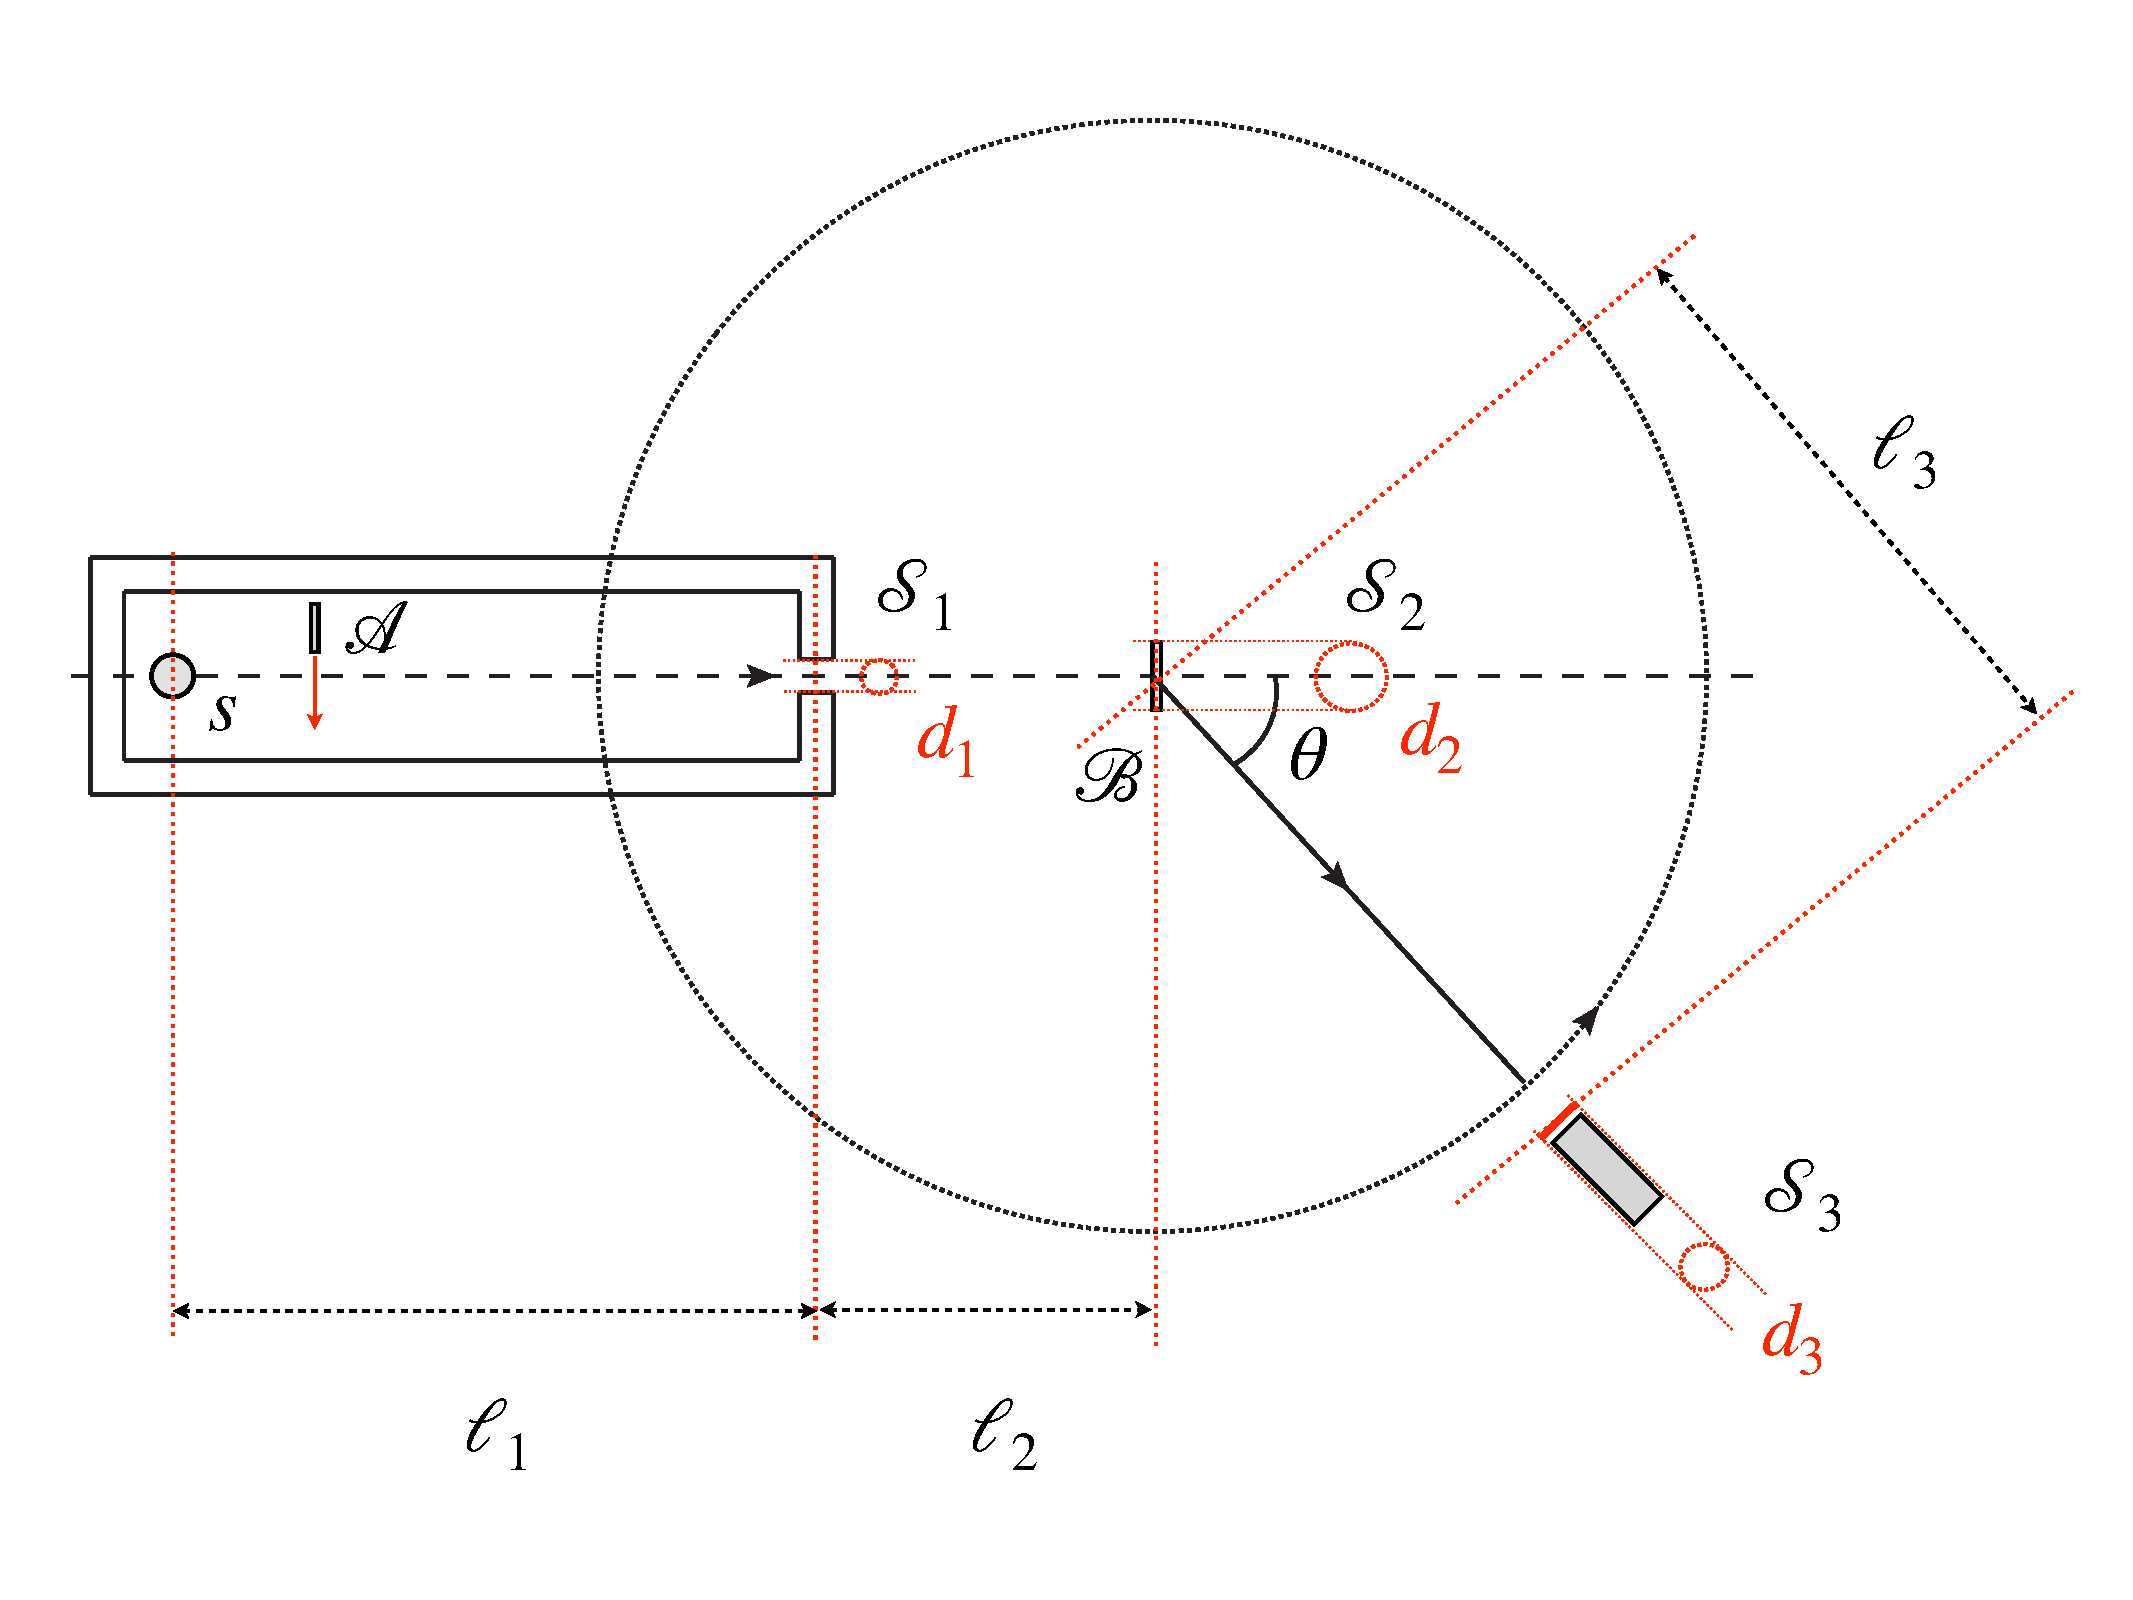
\includegraphics[width=0.85\textwidth]{Scritto-Ic.pdf}
\vskip -0.2cm
\caption{\label{Rutherford} Illustration of the Rutherford experiment.}
\end{figure}


\begin{enumerate}

\item Assuming that the source is point-like, compute the flux of the beam of $\alpha$ particles on the target $B$.

\item Determine the solid angle corresponding to acceptance of the detector. 

\item What is the luminosity of the experiment? 
  
\item The detector is positioned at an angle of 50$^o$, how many particle counts per hour are expected to be recorded? How about when the detector is positioned at an angle of 120$^o$?

\item Determine the  $\beta \gamma$ of $\alpha$ particles of the beam.

\item To verify the energy dependence of the Rutherford scatering cross section, a gold foil within the lead container placed in $\mathcal{A}$ is used to slow the particles of the beam. Determine the thickness of the gold foil needed to obtain a reduction in enregy of 1~MeV (down to a kinetic energy of $E_{\alpha} = 4.5$~MeV).

\item With this thickness compute the effect of multiple scattering on the beam.

\item Assuming that the gold foil is placed very close to the source, can its presence alter the flux of the beam of $\alpha$ particles on the target?

\end{enumerate}
  
{\it Data for $Au$} Atomic mass $M_{Au} = 196.97$~u,  $u =
\SI{1.66054e-24}{g}$,  $\rho_\text{Au} = \SI{19.32}{g/cm^3}$ e $X^0_{Au} = \SI{6.46}{g/cm^{-2}}$

The Avogadro constant is $\mathcal{N}_A = \SI{6.02e23}{mol^{-1}}$.

{\it Energy loss by  ionization and the Bethe-Bloch equation:}

$$
\frac{dE}{\rho dx} =
C\,\frac{Z}{A}\,\frac{z^2}{\beta^2}\,\ln\frac{2m_e\gamma^2\beta^2c^2}{I}
$$

where

$$I \sim Z \times 10 \; {\rm eV} \; \; \; \;  {\rm e} \; \; \; \; C = 4\pi r_e^2 m_e c^2 \mathcal{N}_A = 0.31\ {\rm MeV/ (g . cm^{-2})}$$


{\it Formula for multiple scattering:}

$$\sqrt{\overline{\theta^2_s}} = z \frac{E_s}{pv}\sqrt{\frac{x}{X_0}} \; \;\; \; {\rm e} \; \; \; \;E_s = m_e c^2 \sqrt{\frac{4\pi}{\alpha}} \sim 21\; {\rm MeV}$$


\begin{solution}
  \begin{enumerate}
    
  \item To determine the outgoing flux, we should first calculate the solid angle corresponding to the hole:
  
    $$ \Delta \Omega = \pi (d_1/2)^2 / \ell_1^2 = 0.873 \, 10^{-3} \;
    {\rm sr}$$

  The surface area traversed by the beam on the target will therefore be:
  
    $$ \mathcal{S}_f = \Delta \Omega \times (\ell_1 + \ell_2)^2 = 0.35 \;
    {\rm cm^2} $$

The number of particles per second in  $4\pi$~sr corresponds to $ 5.55 \, 10^{7}$ decays per second,then 

decadimenti per secondo, dunque in $\Delta \omega$ corrispondera a una
frazione $\Delta \omega/4\pi$, dunque circa 3800 particelle $\alpha$ per secondo. Dunque il flusso $\phi$ sarà: 

$$ \phi = 11041 \; {\rm part./(s.cm^2)} $$

\item L'angolo solido del rivelarore corrisponde a:

  $$ \Delta \Omega_{det} = \pi (d_3/2)^2 / \ell_3^2 = 0.873 \,.\, 10^{-3} \;
    {\rm sr}$$ 

\item La luminosità dell'esperimento si esprime in funzione del numero
  di bersagli per il flusso. Il numero di bersagli $N_B$ corrisponde alla
  superficie del fascio $\mathcal{S}_f$ per lo spessore $s_2$ per la
  densità di bersagli:

  $$  N_B = \mathcal{S}_f \times s_2 \times \frac{\rho}{M_{Au} \times u} = 4.1 \, 10^{18} $$

  Dunque la luminosità $\mathcal{L}$ sarà:

  $$\mathcal{L} = N_B \times \phi = 4.6 \, 10^{22} \; {\rm cm^{-2}s^{-1}}$$

\item il numero di conteggi sarà dunque

  $$ N =  \frac{d\sigma}{d\Omega}(\theta) \times \Delta \Omega_{det} \times \Delta t \times \mathcal{L} $$

  Per

  $$r_e^2 \left (\frac{m_ec^2}{4E} \right )^2 = 1.1 \, 10^{-24} \;
  {\rm cm^2} $$

  con $sin (50^o)^4 = 0.032$ si ottiene per ora ($\Delta t = 3600$):

  $$N_{50^o} \sim 5$$

  con $sin (120^o)^4 = 0.562$ si ottiene per ora ($\Delta t = 3600$):
  
  $$N_{120^o} \sim 0.3$$

\item Le particelle $\alpha$ iniziali hanno una velocità di $\beta =
  0.05425$ e $\beta \gamma = 0.05433$. e sono non relativiste,
  possiamo prendere la formula semplificata di Bethe-Bloch e
  otteniamo:

  L'energia persa per ionizzazione in uno spessore $x$ usando la
  formula semplificato (non relativista)

  $$ \Delta E = \rho \times C \times \frac{79}{197} \times \frac{2^2}{0.05425^2} \ln \frac{2 \times 511 \, 10^3 \times 0.05433^2}{790} \times x  = 1~MeV $$

  dunque otteniamo che:

  $$ x = 2.3 \; \mu{\rm m}$$

\item La radice della varianza in angolo di scattering multiplo per
  uno spessore di $x$ sarà, data la formula:

  $$\sqrt{\overline{\theta^2_s}} = z \times \frac{21}{p \times \beta} \sqrt{\dfrac{x}{6.46/19.32}} = 0.1  \; {\rm rad}$$

\item Dato l'angolo di apertura del fascio di $0.5/15. = 0.033$~rad,
  la presenza del foglio d'oro con $\sqrt{\overline{\theta^2_s}} =
  0.1$ avrà dunque un'effetto non trascurabile sul fascio uscente
  riducendo il flusso.
  
\end{enumerate}
\end{solution}